\newpage
\chapter{Излучение темного тела}
\section{Постановка проблемы}

\par Пусть у нас есть некий ящик длиной \textit{l}, нужно найти энергию поля $\rho (w) dw$, где $\rho(w)$ - спектральная плотность. Фактически, это энергия одной характерной моды, умноженная на число мод в интервале \textit{dw}. Разберём, как определить последнее. ЭМ поля представляют собой плоские волны: $\vec{E} \sim e^{i \vec{k} \vec{r}}$. Нас интересуют граничные условия (далее - ГУ) на стенках ящика. Уравнение на поле по пространственным производным - это уравнение второго порядка, поэтому нужно задать либо какое-то значение на стенках, либо значение производной. Но т.к. ящик очень большой, воспользуемся следующим приемом: ГУ наложим периодические
$$f(x+l,y,z)=f(x,y,z) $$
$$f(x,y+l,z)=f(x,y,z) $$
$$f(x,y,z+l)=f(x,y,z) $$
\par То есть получается наш ящик оказывается и не ящиком, а кольцом в 1D, тор - в 2D, тор четырехмерного пространства - в 3D. Данное описание весьма извращенное, но пока мы не интересуемся маленькими ящиками и не хотим думать о модах, которые будут связаны с ГУ на краях ящика (а они могут и быть), то в принципе все равно, какие ГУ накладывать. Конкретные значения $k_i$ дискретны, разные для каждого ГУ, но пока ящик большой, эта дискретность очень маленькая, почти непрерывна, поэтому нам совсем не важен вид ГУ. Подставляем трансляцию на размер ящика \textit{l} в экспоненту, чтобы периодичность сохранилась, фазовый множитель должен быть равен единице, тогда сама фаза $ 2 \pi n$:
$$ k_x l=2 \pi n_x$$
$$ k_y l=2 \pi n_y$$
$$ k_z l=2 \pi n_z$$
\par Небольшой обман: если разделить ящик пополам, поставить новую стенку, решить задачу предыдущую, получить новые ГУ на этой стенке, и здесь уже ГУ начальной задачи важны. Но для более-менее разумных ГУ (нулевые значения функции/производной) это не имеет значения, хотя всегда можно найти ГУ, когда все будет плохо.
\par Вообще \textit{n} - целые числа, а расстояния между соседними \textit{k} это $\frac{1}{l}$, а при $l \shortrightarrow \infty$ у нас $r \shortrightarrow 0$, k - практически непрерывен. В каком интервале  будем его считать? Дисперсионное уравнение дает модуль K есть $|\vec{k}|=\frac{w}{c}$. Если мы фиксируем какую-то \textit{w}, то в пространстве k мы фиксируем сферу радиуса k. Сделаем приращение $ k+d k$. Хотим сосчитать состояния в интервале (w, w+dw), т.е. нужно сосчитать количество дискретных точек K, находящихся между получившимися двумя сферами. 

\begin{wrapfigure}[18]{r}{0.4\linewidth} 
\vspace{-2ex}
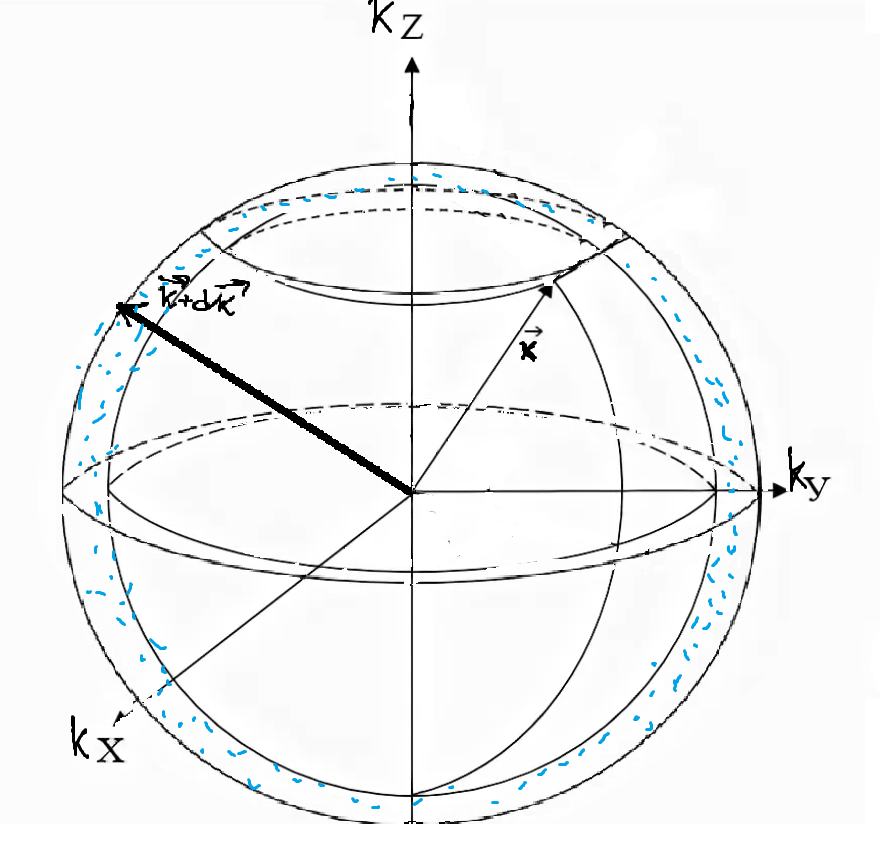
\includegraphics[width=1.2\linewidth]{pictures/3.2.png}
\caption{Координатное пространство k}
\end{wrapfigure}

 \par В нашем случае объем бесконечно малого слоя между сферами $V_{бм}=4 \pi k^2 \Delta k$ (площадь сферы, домноженная на толщину слоя). На каждую точку приходится маленький кубик со стороной $\frac{2 \pi}{l}$, нужно понять, сколько таких кубиков в сферическом слое. Для этого $V_{бм}$ делим на объем кубика \textit{V}. Нам не важно, что есть кубики, вылезающие за рамки слоя, т.к. они очень маленькие, имеют исчезающий размер, поэтому наш ответ верен в асимптотике  $l \shortrightarrow \infty$. Учитывая, что у волн есть 2 поляризации, имеем:
$$ dN = 2 \frac{4 \pi k^2 dk l^3}{(2 \pi)^3} =\frac{k^2dk V}{\pi ^2} $$
\par Подставим $k^2=(\frac{w}{c})^2$, получим $ dN_w =  \frac{w^2 V dw}{c^3 \pi^2} $. Мы сосчитали число колебаний, для поиска $\rho (w) dw$ считаем  $ dN_w $, деленная на единицу объема V и домножаем на некое среднее характерное значение энергии, которая приходится на одну моду $ \overline E_w$ (ибо мы имеем дело с термодинамикой, флуктуации нас не интересуют). Для определения этого среднего необходимо рассмотреть вероятность обнаружения молекулу в интервале скоростей [\textit{V}, \textit{V+dV}]: $f(V)d^3V$, где \textit{f(V)} - функция распределения. Когда имеем дело с термодинамическим равновесием, она имеет определенный вид, зависящий от температуры, хотя обычно обезразмеривают параметр, а так же принимают постоянную k=1: $f(\frac{E_к}{T})$. Распределение Гиббса (хотя вместо E обычно пишут H(p, q)):
$$ f \sim e^{-\frac{E}{T}} $$
$$\overline E_w = \int_{0}^{\infty} Ee^{-\frac{E}{T}}\,dE\ / \int_{0}^{\infty}e^{-\frac{E}{T}} \,dE\ $$
\par Это как бы энергия, взвешенная с числом состояний в интервале dE, а $e^{-\frac{E}{T}} dE$ - не число, а то, чему средняя энергия пропорциональна, поэтому нормируем на него, т.к. интеграл по всем инергиям даст нам единицу. Получим $\overline E_w = T$ (просто взяли интеграл). Закон Релея-Джинса
$$ \rho (w) = \frac{w^2 T}{\pi ^2 c^3} $$
\par Но если бы на сам деле $ \rho (w) \sim w^2 $, то тогда бы темное тело излучало: видимый свет, UV, рентгеновские лучи, $ \gamma $ излучение, но этого не происходит. Аналог темного тела - печь, но многие рядом с печкой находились и оставались живы. Почему?
\par 1896 г. Экспериментально был установлен закон Вина: на больших \textit{w} $$ \lim_{w\to\infty} \rho =e^{-\frac{b w}{T}} $$ В реальности интервал частот регулируется температурой (kT), поэтому существует ограничение полученной ранее несходимости, получившей название UV-катастрофы.



\section{Объяснение UV-катастрофы}

\par Планк утверждал, что проблема в расчете средней энергии моды. Предположение: \textit{E} может принимать только дискретные значения: $E=n E_0$, где \textit{n} - целое число, а $E_0$ что-то непонятное. Вероятность того, что частица имеет энергию $E_0$:   $e^{-n \frac{E_0}{T}}=e^{-n E_0 \beta}$, обозначение $ \beta = \frac{1}{T}$. ЭМ волны принимаются, поглощаются и излучаются стенками, причем это происходит только с дискретными энергиями. Далее вычислим среднюю энергию (в знаменателе сумма из условия нормировки, так же пользуемся суммой геометрической прогрессии):
$$ \overline E = \frac{\sum\limits_{n=0}^ \infty n E_0 e^{-n E_0 \beta}}{\sum\limits_{n=0}^ \infty e^{-n E_0 \beta}} = - \frac{d}{d \beta} ln \sum\limits_{n=0}^ \infty e^{-n E_0 \beta} = - \frac{d}{d \beta} ln \frac{1}{1- e^{-E_0 \beta}} = \frac{E_0}{e^{E_0 \beta} - 1}$$

\begin{wrapfigure}[14]{r}{0.4\linewidth} 
\vspace{-2ex}
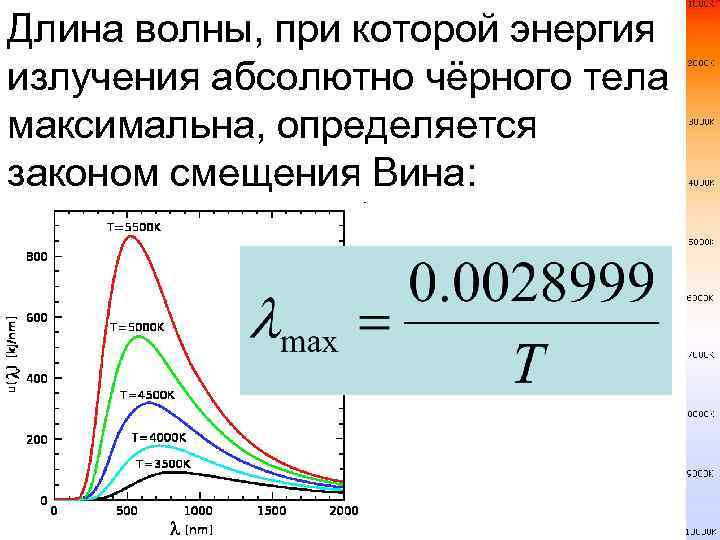
\includegraphics[width=0.8\linewidth]{pictures/3.3.jpg}
\caption{Закон смещения Вина}
\end{wrapfigure}

\par Гипотеза Планка $E_0 = \hbar w$. Видно, что при $ w \shortrightarrow \infty$ экспонента лидирует, получается закон Вина. Тогда при домножении $\overline E$ на число мод все будет хорошо. Из этих соображений можно подобрать $$ \hbar = 1,05 \cdot 10^{-27}эрг \cdot с $$
$$ h= 2 \pi \hbar $$
\par Отсюда $$ \rho (w) = \frac{1}{ \hbar ^2 c^3} \frac{\hbar w^3}{e^{\frac{\hbar w}{kT}}-1} $$ 
\par Максимум данного выражения по частоте наблюдается при $\frac{\hbar w_{max}}{T}=2.84$ (Закон смещения Вина). При низких частотах $ \hbar w < < T$ можно разложить $e^{\frac{\hbar w}{t}} \approx  1 + \frac{\hbar w}{T} $, тогда $ \rho (w) \approx \frac{1}{ \hbar ^2 c^3} \frac{\hbar w^3 T}{\hbar w} = \frac{1}{ \hbar c^3}  w^2 T $ - получили тот же самый ответ, что и раньше для малых частот (учитываем, что $E_0$ мало по сравнению с \textit{T}, а значит, суммирование заменяем интегрированием, т.к. функция на каждом шаге суммирования меняется очень мало). Для больших частот дело обстоит по-другому, как уже было сказано, в той области имеем экспоненциальное спадание, что тоже неплохо. 
\par В качестве развлечения посчитаем полную энергию, получим закон Стефана-Больцмана:
$$ U = \int_{0}^{\infty} \rho _w dw = \int_{0}^{\infty} \frac{1}{\hbar ^2 c^3} \frac{\hbar w^2}{e^{\frac{\hbar w}{T}}-1} dw = \frac{T^4}{\hbar ^2 \pi ^2 c^3} \int_{0}^{\infty} \frac{z^3 dz}{e^z -1} =\frac{T^4}{\hbar ^2 \pi ^2 c^3} \frac{\pi ^4}{15} = \frac{T^4 \pi ^2}{15 \hbar ^2 c^3}$$
\par Словесная формулировка: \textit{Энергия, излучаемая за единицу времени с единицы площади поверхности абсолютно черного тела во всем интервале частот от 0 до $\infty$, пропорциональна четвертой степени абсолютной температуры черного тела.} Вообще, примеров, когда температура контролирует частоту максимального излучения, немало. Сам Стефан применил свой закон к
излучению Солнца и определил температуру его поверхности - 5713 К (современное значение 5780 К, излучает оно больше в диапозоне зеленого света). Полученное им значение температуры Солнца оставалось самым точным в течение всего XIX века. 